% GNUPLOT: LaTeX picture with Postscript
\begingroup
  \makeatletter
  \providecommand\color[2][]{%
    \GenericError{(gnuplot) \space\space\space\@spaces}{%
      Package color not loaded in conjunction with
      terminal option `colourtext'%
    }{See the gnuplot documentation for explanation.%
    }{Either use 'blacktext' in gnuplot or load the package
      color.sty in LaTeX.}%
    \renewcommand\color[2][]{}%
  }%
  \providecommand\includegraphics[2][]{%
    \GenericError{(gnuplot) \space\space\space\@spaces}{%
      Package graphicx or graphics not loaded%
    }{See the gnuplot documentation for explanation.%
    }{The gnuplot epslatex terminal needs graphicx.sty or graphics.sty.}%
    \renewcommand\includegraphics[2][]{}%
  }%
  \providecommand\rotatebox[2]{#2}%
  \@ifundefined{ifGPcolor}{%
    \newif\ifGPcolor
    \GPcolorfalse
  }{}%
  \@ifundefined{ifGPblacktext}{%
    \newif\ifGPblacktext
    \GPblacktexttrue
  }{}%
  % define a \g@addto@macro without @ in the name:
  \let\gplgaddtomacro\g@addto@macro
  % define empty templates for all commands taking text:
  \gdef\gplbacktext{}%
  \gdef\gplfronttext{}%
  \makeatother
  \ifGPblacktext
    % no textcolor at all
    \def\colorrgb#1{}%
    \def\colorgray#1{}%
  \else
    % gray or color?
    \ifGPcolor
      \def\colorrgb#1{\color[rgb]{#1}}%
      \def\colorgray#1{\color[gray]{#1}}%
      \expandafter\def\csname LTw\endcsname{\color{white}}%
      \expandafter\def\csname LTb\endcsname{\color{black}}%
      \expandafter\def\csname LTa\endcsname{\color{black}}%
      \expandafter\def\csname LT0\endcsname{\color[rgb]{1,0,0}}%
      \expandafter\def\csname LT1\endcsname{\color[rgb]{0,1,0}}%
      \expandafter\def\csname LT2\endcsname{\color[rgb]{0,0,1}}%
      \expandafter\def\csname LT3\endcsname{\color[rgb]{1,0,1}}%
      \expandafter\def\csname LT4\endcsname{\color[rgb]{0,1,1}}%
      \expandafter\def\csname LT5\endcsname{\color[rgb]{1,1,0}}%
      \expandafter\def\csname LT6\endcsname{\color[rgb]{0,0,0}}%
      \expandafter\def\csname LT7\endcsname{\color[rgb]{1,0.3,0}}%
      \expandafter\def\csname LT8\endcsname{\color[rgb]{0.5,0.5,0.5}}%
    \else
      % gray
      \def\colorrgb#1{\color{black}}%
      \def\colorgray#1{\color[gray]{#1}}%
      \expandafter\def\csname LTw\endcsname{\color{white}}%
      \expandafter\def\csname LTb\endcsname{\color{black}}%
      \expandafter\def\csname LTa\endcsname{\color{black}}%
      \expandafter\def\csname LT0\endcsname{\color{black}}%
      \expandafter\def\csname LT1\endcsname{\color{black}}%
      \expandafter\def\csname LT2\endcsname{\color{black}}%
      \expandafter\def\csname LT3\endcsname{\color{black}}%
      \expandafter\def\csname LT4\endcsname{\color{black}}%
      \expandafter\def\csname LT5\endcsname{\color{black}}%
      \expandafter\def\csname LT6\endcsname{\color{black}}%
      \expandafter\def\csname LT7\endcsname{\color{black}}%
      \expandafter\def\csname LT8\endcsname{\color{black}}%
    \fi
  \fi
    \setlength{\unitlength}{0.0500bp}%
    \ifx\gptboxheight\undefined%
      \newlength{\gptboxheight}%
      \newlength{\gptboxwidth}%
      \newsavebox{\gptboxtext}%
    \fi%
    \setlength{\fboxrule}{0.5pt}%
    \setlength{\fboxsep}{1pt}%
    \definecolor{tbcol}{rgb}{1,1,1}%
\begin{picture}(9504.00,3744.00)%
    \gplgaddtomacro\gplbacktext{%
      \csname LTb\endcsname%%
      \put(1078,112){\makebox(0,0)[r]{\strut{}$-5000$}}%
      \put(1078,422){\makebox(0,0)[r]{\strut{}$0$}}%
      \put(1078,732){\makebox(0,0)[r]{\strut{}$5000$}}%
      \put(1078,1042){\makebox(0,0)[r]{\strut{}$10000$}}%
      \put(1078,1352){\makebox(0,0)[r]{\strut{}$15000$}}%
      \put(1078,1662){\makebox(0,0)[r]{\strut{}$20000$}}%
      \put(1078,1973){\makebox(0,0)[r]{\strut{}$25000$}}%
      \put(1078,2283){\makebox(0,0)[r]{\strut{}$30000$}}%
      \put(1078,2593){\makebox(0,0)[r]{\strut{}$35000$}}%
      \put(1078,2903){\makebox(0,0)[r]{\strut{}$40000$}}%
      \put(1078,3213){\makebox(0,0)[r]{\strut{}$45000$}}%
      \put(1078,3523){\makebox(0,0)[r]{\strut{}$50000$}}%
      \put(1210,-680){\rotatebox{90}{\makebox(0,0)[l]{\strut{}306.000}}}%
      \put(2526,-680){\rotatebox{90}{\makebox(0,0)[l]{\strut{}307.000}}}%
      \put(3637,-680){\rotatebox{90}{\makebox(0,0)[l]{\strut{}307.844}}}%
      \put(3836,-680){\rotatebox{90}{\makebox(0,0)[l]{\strut{}307.995}}}%
      \put(4274,-680){\rotatebox{90}{\makebox(0,0)[l]{\strut{}308.328}}}%
      \put(4526,-680){\rotatebox{90}{\makebox(0,0)[l]{\strut{}308.520}}}%
      \put(4808,-680){\rotatebox{90}{\makebox(0,0)[l]{\strut{}308.734}}}%
      \put(5159,-680){\rotatebox{90}{\makebox(0,0)[l]{\strut{}309.000}}}%
      \put(6475,-680){\rotatebox{90}{\makebox(0,0)[l]{\strut{}310.000}}}%
      \put(7791,-680){\rotatebox{90}{\makebox(0,0)[l]{\strut{}311.000}}}%
      \put(9107,-680){\rotatebox{90}{\makebox(0,0)[l]{\strut{}312.000}}}%
    }%
    \gplgaddtomacro\gplfronttext{%
      \csname LTb\endcsname%%
      \put(209,1817){\rotatebox{-270}{\makebox(0,0){\strut{}I (a.u.)}}}%
      \put(5158,-1098){\makebox(0,0){\strut{}$\lambda$ (nm)}}%
    }%
    \gplbacktext
    \put(0,0){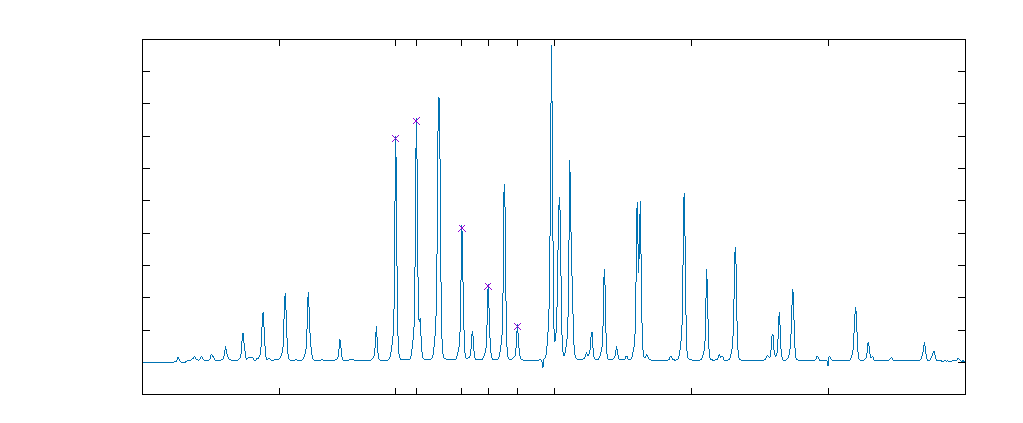
\includegraphics[width={475.20bp},height={187.20bp}]{OH7_data}}%
    \gplfronttext
  \end{picture}%
\endgroup
